\documentclass{article}
\usepackage[english]{babel}
\usepackage[letterpaper,top=2cm,bottom=2cm,left=3cm,right=3cm,marginparwidth=1.75cm]{geometry}
\usepackage{amsmath}
\usepackage{graphicx}
\usepackage[colorlinks=true, allcolors=blue]{hyperref}

\title{\textbf{CS456: Algorithm Design and Analysis}}
\author{Elikem Asudo Tstatsu Gale-Zoyiku}
\date{9th Februrary, 2024}

\begin{document}
\maketitle
\begin{center}
    \begin{large}
        \textbf{Assignment 2\\}
    \end{large}
\end{center}
\newpage
\section*{Question 1}
\begin{enumerate}
    \item Constant Factor in Execution Time:
          The data shows that the count, representing the algorithm's execution time, consistently falls within a narrow range (between 11 and 13 times the input size) across various input sizes.
          \begin{itemize}
              \item For instance, with an input size of 2000, the count is 24,303, and with an input size of 3000, the count is approximately 39,992.
              \item Calculating the ratio of count to input size for each data point reveals a nearly constant factor, around 12, regardless of the input size.
              \item Consider the data point with an input size of 1000: Count is approximately 11,966.
                    Calculating the ratio of count to input size: \( \frac{11966}{1000} \approx 11.966 \).
                    Similarly, for the data point with an input size of 2000: Count is approximately 24,303, and the ratio is \( \frac{24303}{2000} \approx 12.152 \).
                    Despite doubling the input size from 1000 to 2000, the ratio remains close to 12, indicating a nearly constant factor.
          \end{itemize}

    \item Linear Relationship:
          \begin{itemize}
              \item Doubling the input size approximately doubles the count, demonstrating a linear relationship between the input size and the count. For example, when the input size increases from 1000 to 2000, the count roughly doubles from 11,966 to 24,303.
              \item Take the example of doubling the input size from 2000 to 4000.
                    With an input size of 2000, the count is around 24,303, and with an input size of 3000, the count is approximately 53,010.
                    The ratio of counts is \( \frac{53010}{24303} \approx 2 \).
                    Doubling the input size approximately doubles the count, demonstrating a linear relationship.
                    This consistent doubling behavior across different input sizes indicates that the execution time scales linearly with the size of the input data.
          \end{itemize}
          These two observations suggest that the algorithm's execution time has a linear relationship with the input size, with a nearly constant factor. This implies that the algorithm has a time complexity of \( O(n) \), where \( n \) is the input size.

    \item Graphical Representation:

          To visually illustrate these observations, the data points have been plotted on a graph with the input size on the x-axis and the count on the y-axis.
          The graph clearly depicts a linear relationship, where the data points form a straight line with a positive slope.
          This linear behavior on the graph further reinforces the hypothesis of linear time complexity (O(n)) for the algorithm, as it demonstrates that the execution time increases linearly with the input size.
          The graph can be seen below:
          \begin{center}
              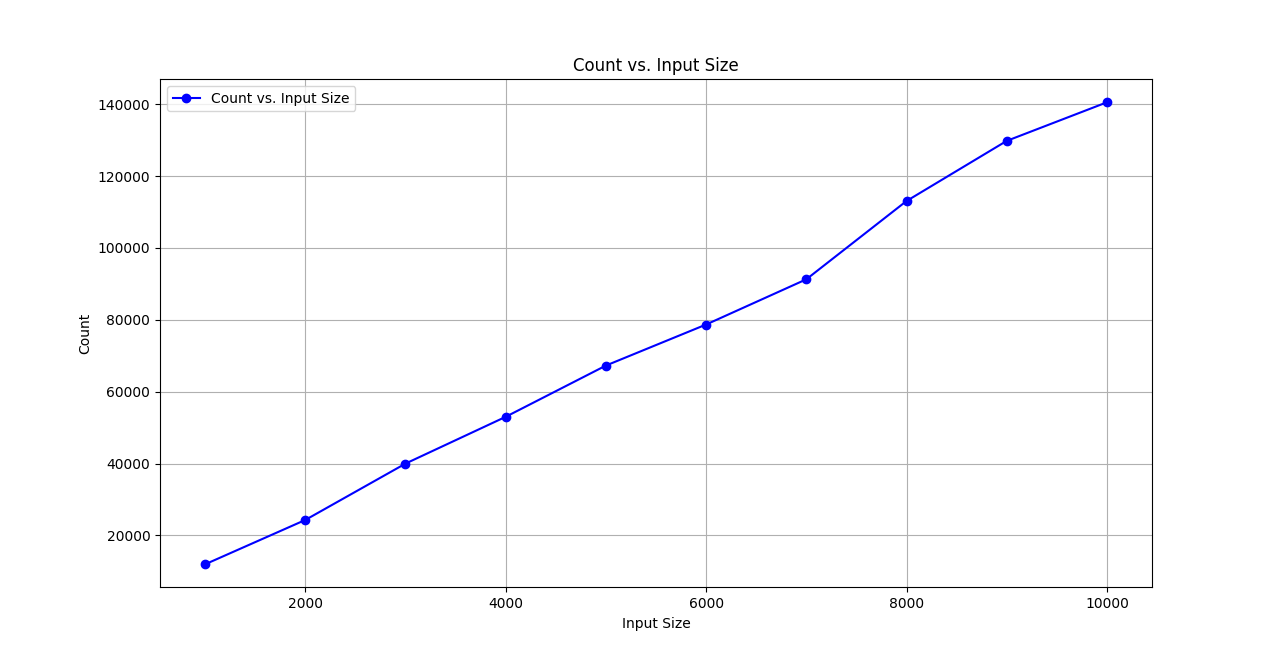
\includegraphics[width=0.9\textwidth]{graph.png}
          \end{center}
\end{enumerate}
\newpage
\section*{Question 2}
\subsection*{a}This algorithm computes the minimum value in an array of real numbers.
It recursively searches for the minimum value by comparing elements of the array.
The base case is when the array contains only one element, in which case the algorithm returns that element as the minimum value.
Otherwise, it recursively finds the minimum value in the subarray A[0 .. n-2] and compares it with the last element of the array (A[n-1]).
If the minimum value from the subarray is less than or equal to the last element, it returns the minimum value from the subarray.
Otherwise, it returns the last element of the array as the minimum value.

\subsection*{b}
Let the basic operation count of the algorithm as T(n), where n is the size of the input array A.

The basic operations in this algorithm are comparisons and recursive calls.
\begin{itemize}
    \item Comparisons: There are (n-1) comparisons made in the worst case scenario when checking each element of the array to find the minimum value.
    \item Recursive Calls: The algorithm makes one recursive call for each element of the array except for the first one. Therefore, there are (n-1) recursive calls in total.
\end{itemize}
Hence, the recurrence relation for the algorithm is:
\[ T(n) = T(n-1) + (n-1) \]
Solving:
\[ T(n) = T(n-1) + (n-1) \]
\[ = [T(n-2) + (n-2)] + (n-1) \]
\[ = T(n-2) + (n-2) + (n-1) \]
\[ = T(n-3) + (n-3) + (n-2) + (n-1) \]
\[ \vdots \]
\[ = T(n-(n-1)) + (n-(n-1)) + \dots + (n-3) + (n-2) + (n-1) \]
\[ = T(1) + 1 + 2 + 3 + \dots + (n-1) \]

The sum of the first \( n-1 \) natural numbers can be expressed as \( \frac{n(n-1)}{2} \), so:
\[ T(n) = T(1) + \frac{n(n-1)}{2} \]
The base case is when \( n = 1 \) and the algorithm simply returns the single element of the array, \( T(1) = c \) where c is a constant time operation so T(1) is dropped from the equation.
\[ T(n) = \frac{n(n-1)}{2} \]
Therefore, the closed form format for the recurrence relation of the algorithm's basic operation count is \( T(n) = \frac{n(n-1)}{2} \).

\subsection*{Prooving by induction:}
\begin{enumerate}
    \item Base Case (n = 1):
          When \( n = 1 \), \( T(1) = 0 \) (as there are no comparisons or recursive calls needed for an array of size 1).
          Therefore, the base case holds true.

    \item Inductive Step:
          Assume that the closed form solution \( T(k) = \frac{k(k-1)}{2} \) holds for some arbitrary integer \( k \geq 1 \).
          and prove that \( T(k+1) = \frac{(k+1)k}{2} \).

          Using the recurrence relation:
          \[ T(k+1) = T(k) + k \]

          Substituting the assumed closed form solution for \( T(k) \):
          \[ T(k+1) = \frac{k(k-1)}{2} + k \]

          Simplifying:
          \[ T(k+1) = \frac{k(k-1)}{2} + \frac{2k}{2} \]
          \[ T(k+1) = \frac{k^2 - k + 2k}{2} \]
          \[ T(k+1) = \frac{k^2 + k}{2} \]
          \[ T(k+1) = \frac{(k+1)k}{2} \]

          Hence, the closed form solution holds for \( k+1 \).

\end{enumerate}
Therefore, the recurrence relation has the closed form solution \( T(n) = \frac{n(n-1)}{2} \).
\newpage
\section*{Question 3}
\newpage
\section*{Question 4}
\newpage
\section*{Question 5}
\newpage
\section*{Question 6}
\newpage


\end{document}
